\section{直流电动机}\label{sec:10-10}

电动机是把电能转化为机械能的机器。用直流电源\footnotemark 供电的电动机叫做\textbf{直流电动机}。
直流电动机就是利用通电线圈能在磁场里转动的原理制成的。
在图 \ref{fig:10-41} 的实验中我们看到,通电线圈在磁场里能够转动,但转到平衡位置时摆动几下就停了下来,
而直流电动机要连续转动下去才行,怎样才能办到这一点呢?
\footnotetext{电流分直流和交流两种。
方向不变的电流叫直流电,方向作周期性变化的电流叫交流电(参看后面的第十三节)。
能供给直流电的电源叫直流电源。 电池、直流发电机都是直流电源。}

在图 \ref{fig:10-41} 中,如果在线圈由于惯性刚转过平衡位置时,立刻改变线圈中的电流方向,
那么线圈就能够继续转动下去。可见,要造成直流电动机,
必须设法使线圈一到平衡位置就能自动地改变线圈里的电流方向。
能够完成这一任务的装置叫做\textbf{换向器}。

彩图5 \footnote{我找到的原书扫描版PDF中,仅有3个彩图。所以这里没有办法显示。其它的彩图也是这个原因。}
表示出了直流电动机的构造和工作原理。线圈 $abcd$ 和换向器 $E$、$F$ 都装在转动轴上。
换向器$E$、$F$ 是两个铜制的半环,它们彼此绝缘,并且都跟转动轴绝缘。
$A$、$B$ 是电刷,它们跟换向器接触,使电源和线圈组成闭合电路。
电流是由直流电源经过电刷、换向器流入线圈的。

线圈在图甲所示的位置的时候,换向器的半环 $E$ 跟电刷 $B$ 接触,
半环 $F$ 跟电刷 $A$ 接触,线圈中的电流从 $E$ 流向 $F$。
根据左手定则知道,这时线圈沿着顺时针方向转动。
当线圈转到平衡位置的时候(图乙),两电刷恰好接触两半环间的绝缘部分,
线圈由于惯性还能稍微转过一些,而线圈稍微转过平衡位置,两个半环接触的电刷就调换了,
变成半环 $F$ 跟电刷 $B$ 接触,半环 $E$ 跟电刷 $A$ 接触,
线圈中的电流也就变成从 $F$ 流向 $E$,于是线圈继续沿顺时针方向转动(图丙)。
这样,每当线圈稍微转过平衡位置时,换向器就自动改变线圈中电流的方向,线圈也就不停地转动下去。

如果把电动机的转轴跟水泵或别的工作机的轴连起来,电动机转动时就可以带动水泵抽水或别的工作机工作。
这时电能就转化成机械能。实际的直流电动机,为了能带动工作机平稳地运转,线圈有很多匝,
并且嵌在圆柱形铁心上,组成转子。换向器也由许多铜片组成(图 \ref{fig:10-42})。

\begin{figure}[htbp]
    \centering
    \begin{minipage}{7cm}
    \centering
    \vspace{3cm}
    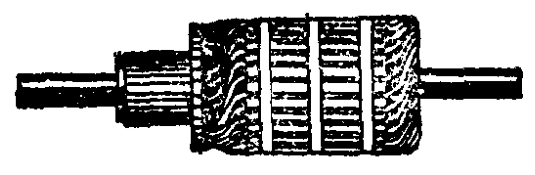
\includegraphics[width=6cm]{../pic/czwl2-ch10-42}
    \caption{}\label{fig:10-42}
    \end{minipage}
    \qquad
    \begin{minipage}{7cm}
    \centering
    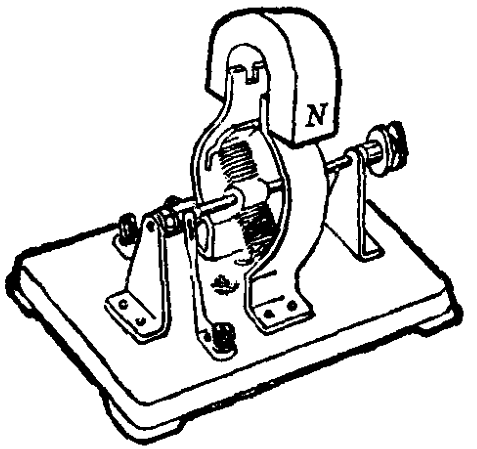
\includegraphics[width=6cm]{../pic/czwl2-ch10-43}
    \caption{}\label{fig:10-43}
    \end{minipage}
\end{figure}

跟热机比较,电动机有许多优点。
电动机的开动和停止都比热机方便,只要用电键把它的电路接通或切断就行了。
电动机的构造也比热机简单,制造起来比较便宜,占的地方比较小。
此外电动机的效率也比热机高得多。
电动机广泛应用在电车、电力机车(彩图6)以及轧钢机、起重机(彩图7)等方面。
